\documentclass{article}

%\documentclass[conference]{IEEEtran}
%\documentclass{article}
\usepackage[letterpaper,margin=1in]{geometry}

\usepackage[utf8]{inputenc}
\usepackage{fancyhdr}
\usepackage{mathtools}
\usepackage{amsmath}
\usepackage{graphicx}
\usepackage{textcomp}
\usepackage[table,xcdraw]{xcolor}
\usepackage{mathtools}
\usepackage{empheq}
\newcommand*\widefbox[1]{\fbox{\hspace{2em}#1\hspace{2em}}}
\usepackage{color}


\usepackage{hyperref}
\usepackage{titling}

\renewcommand\maketitlehooka{\null\mbox{}\vfill}
\renewcommand\maketitlehookd{\vfill\null}
\usepackage{float}
\usepackage{steinmetz}
\usepackage{xspace}


\newcommand{\MATLAB}{\textsc{Matlab}\xspace}
\usepackage{chngcntr}

% Bibliograpy
\usepackage[english]{babel}
%\usepackage{cite}
\usepackage[
backend=biber,
style=ieee,
]{biblatex}

\addbibresource{References.bib} %Imports bibliography file


\counterwithin*{equation}{section}
\counterwithin*{equation}{subsection}

% Listings
\usepackage{listings}

% Listings Colors
\definecolor{codegreen}{rgb}{0,0.6,0}
\definecolor{codegray}{rgb}{0.5,0.5,0.5}
\definecolor{codepurple}{rgb}{0.58,0,0.82}
\definecolor{backcolour}{rgb}{0.95,0.95,0.92}

\lstdefinestyle{mystyle}{
	backgroundcolor=\color{white},   
	commentstyle=\color{codegreen},
	keywordstyle=\color{blue},
	numberstyle=\tiny\color{codegray},
	stringstyle=\color{codepurple},
	basicstyle=\footnotesize,
	breakatwhitespace=false,         
	breaklines=true,                 
	captionpos=b,                    
	keepspaces=true,                 
	numbers=left,                    
	numbersep=5pt,                  
	showspaces=false,                
	showstringspaces=false,
	showtabs=false,                  
	tabsize=2,
	frame=leftline
}


\lstset{style=mystyle}

% ASSIGNMENT NAME GOES HERE
\def \myAssignmentName {ECE 5013: Radar Design Project}
% header/footer formatting
\pagestyle{fancy}
\fancyhf{}

\chead{\myAssignmentName}
\rhead{04/23/2020}
\rfoot{\thepage}

%Title Page
\title{\myAssignmentName}
\author{Matt Gambill \\ \href{mailto:gambill.46@osu.edu}{\textcolor{blue}{\underline{gambill.46@osu.edu}}} \and  Enzo Ocampo\\  \href{mailto:ocampo.29@osu.edu}{\textcolor{blue}{\underline{ocampo.29@osu.edu}}}}
\date{April 23, 2020}
% CONTENT

\begin{document}
% MAKE COVER PAGE
\begin{titlingpage}
\maketitle
\end{titlingpage}
\tableofcontents

\listoffigures

\listoftables
\newpage

% Insert Content Here
% set equation numbers to section.eq#
\renewcommand{\theequation}{\thesubsection.\arabic{equation}}

% Begin Sections
\section{Introduction and System Model}
In this final project, our group will be studying a MISO (Multi-Input Single Output) Pulse Doppler System. The given radar system has 2 transmit and 1 receiving antenna and operates at a center frequency of 10.5 GHz. The total system bandwidth is 125 MHz. The two transmitters using and down chirp waveforms are given by equation \ref{eq:1}.

\begin{equation}
    s(t) = A_c e^{j(2\pi f_c t \pm \pi \frac{\beta_0}{\tau_0} p_{\tau_0}(t)}
    \label{eq:1}
\end{equation}

Where AC has a transmit power of 20 dBm and $\beta_{0} = 120 MHz$ is the sweep bandwidth. $p_{\tau0}$ is a rectangular pulse, defined as $p_{\tau0} = 1$ for $-\frac{\tau_{0}}{2} \leq t \leq \frac{\tau_{0}}{2}$ and zero otherwise with  $\tau = 80 \mu s$. The pulse repetition frequency of the system is given by 1 kHz. The coherent processing interval is assumed to be 64 pulses. The two transmit antennas are placed $\lambda/2$ apart and have a beam-width of 60 degrees, with 3 dBi gain. The noise figure of the system is 8 dB.

\section{Theory Review}
\subsection{LFM Waveform}
The ambiguity function shows the response from a target whose delay and Doppler is $\Delta t$ and $ \Delta f_d$  away from a target of interest, as denoted by the Equation \ref{eq:LFM1}.

\begin{equation}
    \chi(\Delta t, \Delta f) = \int_{-\infty}^{\infty} x(t) x^*(t-\Delta t)e^{j(2\pi \delta ft)} dt
    \label{eq:LFM1}
\end{equation}

Where the output of the matched filter to an interfering target for the filter is designed for a target at $t = 0$ and $f_d = 0$. The ambiguity function is the magnitude of the complex response, as described in the following Equation \ref{eq:LFM2}.

\begin{equation}
    A(\Delta t, \Delta f) = \lvert x(\Delta t, \Delta f) \rvert
    \label{eq:LFM2}
\end{equation}

Where $\chi(\Delta t, \Delta f)$ is the complex ambiguity function and $\lvert \chi(\Delta t, \Delta f) \rvert$ is the ambiguity function, respectively.

\subsection{Match Filtering}
Similar to the ambiguity function for the LFM waveform, the matched filter response from a target whose delay and Doppler is is $\tau$ and $\nu$ away from target of interest, seen in Equation \ref{eq:MF1}.

\begin{equation}
    \chi(\Delta t, \Delta f) = \int_{-\infty}^{\infty} x(t)x^*(t-\tau)e^{j(2\pi\nu\tau)} dt
    \label{eq:MF1}
\end{equation}

The ambiguity function for matched filtering is the magnitude of the complex response, seen in Equation \ref{eq:MF2}.

\begin{equation}
    A(\tau, \nu) = \lvert \chi(\tau, \nu) \rvert
    \label{eq:MF2}
\end{equation}

In ideal conditions, the match filter should only respond to the delay and Doppler $( \tau_0, \nu_0)$ it was designed for. The output will be non-zero for targets that are at a similar delay and Doppler bin $( \tau_0 + \tau, \nu_0 + \nu)$. $A(\tau, \nu)$ denotes the magnitude of the matched filter output of a target $( \tau, \nu)$ away in both delay and Doppler.

\subsection{Doppler Processing}
There are two major classes of Doppler processing: Moving Target Identification (MTI) and Pulse Doppler Processing. Moving Target Identification is where the pulse-to-pulse signal is processed
entirely in time domain. This is typically used for Low PRF( ambiguous doppler, unambiguous range). It has low computational cost and is primarily focused on removing stationary clutter. Pulse Doppler Processing is where the pulse-to-pulse signal is processed in the frequency domain. This is common in cases of High PRF (unambiguous doppler, ambiguous range) where digital signal processing is applied to complex baseband samples. This leads to a higher signal-to-interference ratio. For this project, we'll also be looking at the method of I-Q Sampling, detailed in equation \ref{eq:DP1}.

\begin{equation}
    x(t) = Ae^{j\phi} \sum_{n} p(t - t_d - nT_p)e^{j(2\pi f_d t)}
    \label{eq:DP1}
\end{equation}

where
\begin{equation} 
    t_d = \frac{2R_0}{c} 
    \label{eq:DP2} 
\end{equation}  

and 
\begin{equation} 
    f_d = \frac{2v}{\lambda} 
    \label{eq:DP3} 
\end{equation}
which leads to match filtering the received signal and obtaining N samples over N pulses, denoted in equation \ref{eq:DP4}.

\begin{equation}
    y[n] = Ae^{j(2\phi)} R_{pp} (0) e^{j2\pi f_d T_pn}e^{j2\pi f_d T_d} = A_c e^{2\pi f_d T_pn} = A_c e^{j2\pi f_dn}
    \label{eq:DP4}
\end{equation}

\section{Simulation Results}
\subsection{RADAR Returns}
 A simulator was built to model the RADAR system. The single pulse response for a 30 meter range and $-10^{\circ}$ azimuth was plotted in Figures \ref{fig:Tx1NR} and \ref{fig:Tx2NR}. SNR was measured to be consistent with the RADAR Range Equation.
\begin{figure}[H]
    \centering
    \includegraphics[width=0.75\textwidth]{figures/Tx1NoisyReturns.pdf}
    \caption{Tx1 Noisy Returns}
    \label{fig:Tx1NR}
\end{figure}

\begin{figure}[H]
    \centering
    \includegraphics[width=0.75\textwidth]{figures/Tx2NoisyReturns.pdf}
    \caption{{Tx2} Noisy Returns}
    \label{fig:Tx2NR}
\end{figure}

\subsection{Ambiguity Function Plots}
The Ambiguity functions and their outputs are displayed in the following figures.
\begin{figure}[H]
    \centering
    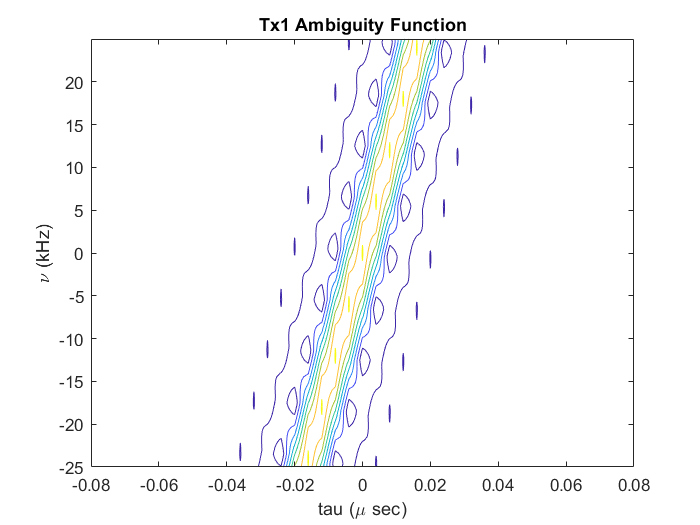
\includegraphics[width=0.75\textwidth]{figures/ambiguityFunction_1pulse_Tx1_2D.png}
    \caption{Ambiguity Function 1 pulse Tx1 2D}
    \label{fig:AF1_Tx1_2D}
\end{figure}

\begin{figure}[H]
    \centering
    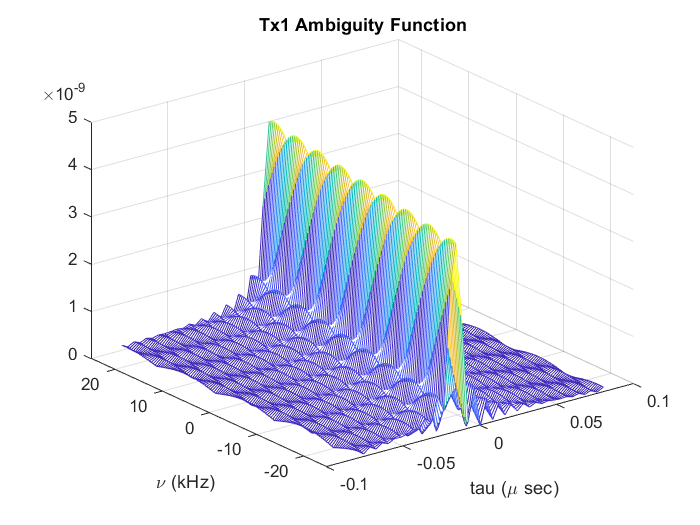
\includegraphics[width=0.75\textwidth]{figures/ambiguityFunction_1pulse_Tx1_3D.png}
    \caption{Ambiguity Function 1 pulse Tx1 3D}
    \label{fig:AF1_Tx1_3D}
\end{figure}

\begin{figure}[H]
    \centering
    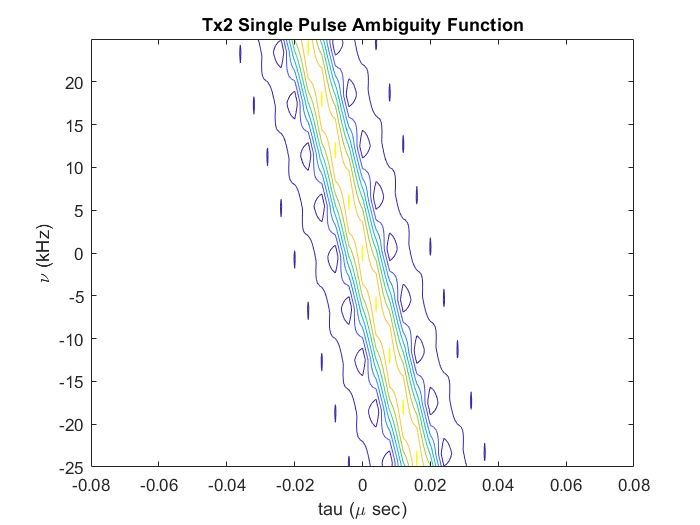
\includegraphics[width=0.75\textwidth]{figures/ambiguityFunction_1pulse_Tx2_2D.png}
    \caption{Ambiguity Function 1 pulse Tx2 2D}
    \label{fig:AF1_Tx2_2D}
\end{figure}

\begin{figure}[H]
    \centering
    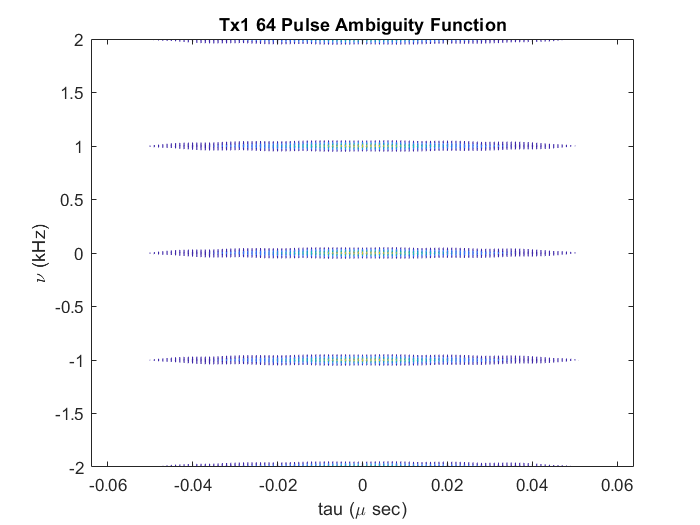
\includegraphics[width=0.75\textwidth]{figures/ambiguityFunction_64pulse_Tx1_2D.png}
    \caption{Ambiguity Function 64 pulse Tx1 2D}
    \label{fig:AF64_Tx1_2D}
\end{figure}

\begin{figure}[H]
    \centering
    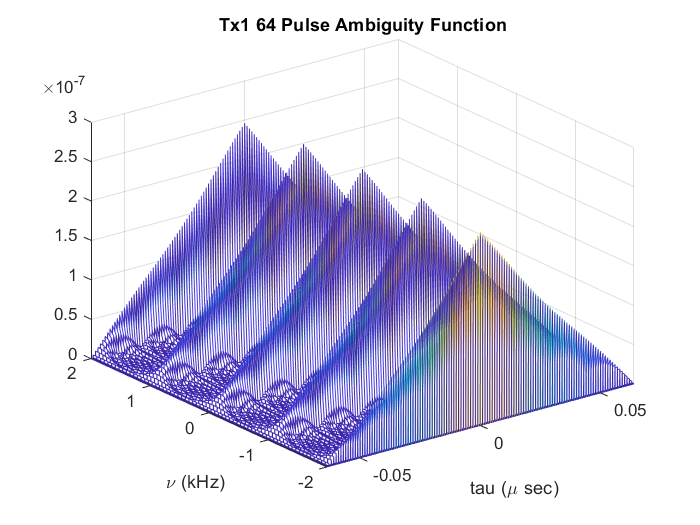
\includegraphics[width=0.75\textwidth]{figures/ambiguityFunction_64pulse_Tx1_3D.png}
    \caption{Ambiguity Function 64 pulse Tx1 3D}
    \label{fig:AF64_Tx1_3D}
\end{figure}

\begin{figure}[H]
    \centering
    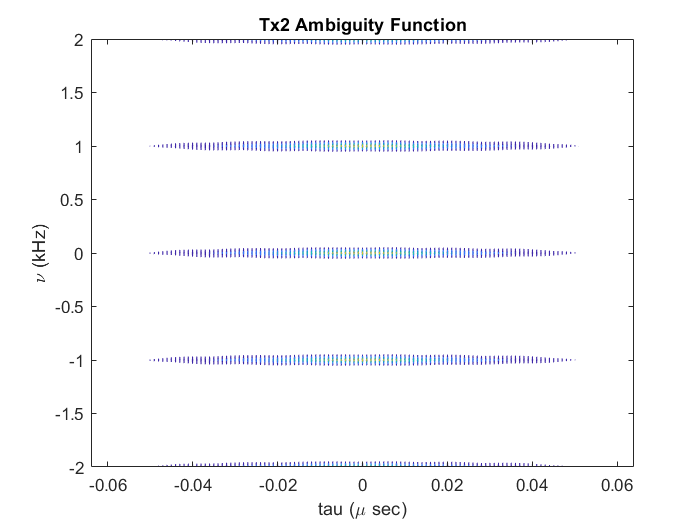
\includegraphics[width=0.75\textwidth]{figures/ambiguityFunction_64pulse_Tx2_2D.png}
    \caption{Ambiguity Function 64 pulse Tx2 2D}
    \label{fig:AF64_Tx2_2D}
\end{figure}

\begin{figure}[H]
    \centering
    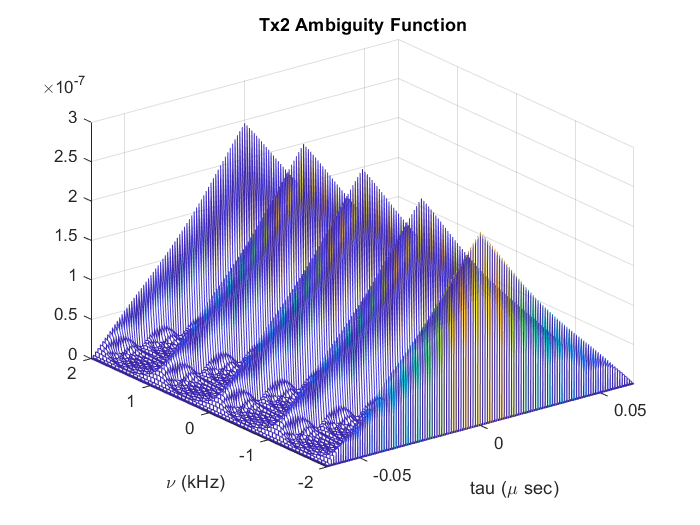
\includegraphics[width=0.75\textwidth]{figures/ambiguityFunction_64pulse_Tx2_3D.png}
    \caption{Ambiguity Function 64 pulse Tx2 3D}
    \label{fig:AF64_Tx2_3D}
\end{figure}

\subsection{Simulation of a Moving Target}
A simulator was developed to model a moving target traveling from $\theta = -10^{\circ}$ to $\theta = 10^{\circ}$ at a velocity of $10 \frac{m}{s}$. Code listings are provided in Appendix A. The code runs over 15 coherent processing intervals (CPI).The code provides range,and  azimuth predictions, as well as a Range-Doppler Map for each CPI. 

Range is calculated by finding the maximum(s) of the range-Doppler map. The maximum provides a delay time for each \verb|Tx| channel. Since the channels are separated by a distance of $\lambda/2$, range and azimuth can be predicted by Equations \ref{eq:sub0}, which is derived in Appendix B.

\begin{subequations}
\begin{empheq}[]{align}
    \begin{bmatrix} 8 c_1 & -4d \\ 8 c_2 & 4d \end{bmatrix} \begin{bmatrix} R \\ y \end{bmatrix} &= \begin{bmatrix} 4 c_1^2 - d^2\\ 4c_2 -d^2 \end{bmatrix} \\
    \mathbf{A x} &= \mathbf{b}\\
    \sin^{-1}(\frac{y}{R}) &= \theta\\
    c*t_{d \, \mathrm{tx_1}} &= c_1 \label{eq:sub1g} \\
    c*t_{d \, \mathrm{tx_2}} &= c_2 \label{eq:sub1h} \\
    d & = \lambda/2 \label{sub1i}
\end{empheq}
\label{eq:sub0}
\end{subequations}

Attached to this report, Range-Doppler Maps are shown in a GIF, and Table 1 shows the predicted normalized Range, Velocity, and Azimuth Error. Range error is 2-3\% while Azimuth and Velocity error are quite high. Analysis reveals that the error is due to range resolution. The target moves less than a meter in Range at a distance of 25 meters in the $x$ direction from the receiver. The RADAR as currently designed is not capable of resolving the target at the specified distances. Potential changes to simulator to reduce error include changing the sweep bandwidth for the LFM waveform or changing how match filtering is implemented.

\begin{table}
\centering
\resizebox{0.5\textwidth}{!}{
\begin{tabular}{|c|c|c|}
\hline
Range Error & Azimuth Error & Velocity Error \\
\hline
0.02 & -1.00 & 1.00 \\
\hline
0.02 & -1.00 & 1.00 \\
\hline
0.02 & -1.00 & 1.00 \\
\hline
0.03 & -1.00 & 1.00 \\
\hline
0.03 & -1.00 & 1.00 \\
\hline
0.03 & -1.00 & 1.00 \\
\hline
0.03 & -1.00 & 1.00 \\
\hline
0.03 & - & 1.00 \\
\hline
0.03 & 1.00 & 1.00 \\
\hline
0.03 & 1.00 & 1.00 \\
\hline
0.03 & 1.00 & 1.00 \\
\hline
0.03 & 1.00 & 1.00 \\
\hline
0.02 & 1.00 & 1.00 \\
\hline
0.02 & 1.00 & 1.00 \\
\hline
0.02 & 1.00 & 1.00 \\
\hline
\end{tabular}}
\caption{Normalized Error For Each CPI}
\label{table:Problem 3}
\end{table}


\newpage
\section{Results from Measured Data}
Data was acquired from Dr. Emre Ertin. Figure \ref{fig:dataMap}  shows the Doppler Range maps. Code for the plot can be found in Appendix A. An animated GIF is also attached with this report.
\begin{figure}[H]
    \centering
    \includegraphics[width=0.75\textwidth]{figures/dataPlot_1.pdf}
    \caption{Data Range Doppler Map}
    \label{fig:dataMap}
\end{figure}

\section{Acknowledgments}
Dr. Ertin's Lecture Slides \cite{lecSlides} were invaluable to our report.
% bibliography
\printbibliography

\appendix
\section{Code}

\lstinputlisting[language=Octave, caption={Problem 4 Simulation Code}]{./code/PT4SIMUALATION.m}
\lstinputlisting[language=Octave, caption={radarSimulator Code}]{./code/radarSimulator.m}
\lstinputlisting[language=Octave, caption={getPos Code}]{./code/getPos.m}
\lstinputlisting[language=Octave, caption={rpulse Code}]{./code/rpulse.m}
\lstinputlisting[language=Octave, caption={readData Code}]{./code/readData.m} \label{lst:dataCode}

\newpage

\section{Derivations}
\subsection{getPos Function Derivation}
The following section details how the \MATLAB function \verb|getPos| was derived. Equations \ref{eq:sub1a} to \ref{eq:sub1f} describe the geometry shown in Figure \ref{fig:probGeometry}.

\begin{figure}[H]
    \centering
    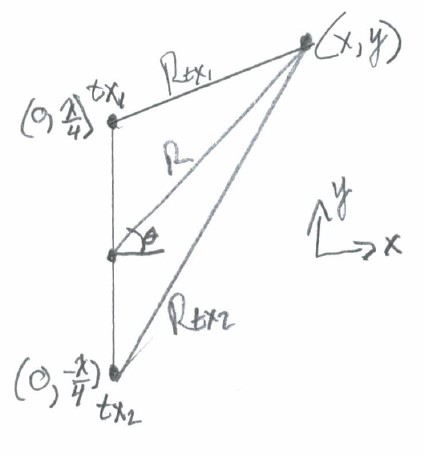
\includegraphics[width=0.25\textwidth]{figures/geometry.jpg}
    \caption{Problem Geometry}
    \label{fig:probGeometry}
\end{figure}

\begin{subequations}
\begin{empheq}{align}
    (y- \frac{\lambda}{4})^2 +x^2 &= R_{\mathrm{tx_1}}^2 \label{eq:sub1a} \\ 
    (y+ \frac{\lambda}{4})^2 +x^2 &= R_{\mathrm{tx_2}}^2  \label{eq:sub1b}\\
    x^2 + y^2 &= R^2  \label{eq:sub1c}\\
    \tan^{-1}(\frac{y}{x}) &= \theta \label{eq:sub1d} \\
    R + R_{\mathrm{tx_1}} &=  c_1 \label{eq:sub1e}\\
    R + R_{\mathrm{tx_2}}& =  c_2  \label{eq:sub1f} \\
    c*t_{d \, \mathrm{tx_1}} &= c_1 \label{eq:sub1g} \\
    c*t_{d \, \mathrm{tx_2}} &= c_2 \label{eq:sub1h} \\
    d & = \lambda/2 \label{sub1i}
\end{empheq}
\label{eq:sub1}
\end{subequations}

Where $c$ is the speed of light, $t_{d \, \mathrm{tx_1}}$ is the delay time from \texttt{TX1}, $t_{d \, \mathrm{tx_2}}$ is the delay time from \texttt{TX2}, and $\lambda$ is the wavelength. From equations \ref{eq:sub1e} and \ref{eq:sub1f}, equations \textbf{\ref{eq:sub2}} are derived. 

\begin{subequations}
\begin{empheq}{align}
    R_{\mathrm{tx_1}} = c_1 - R   \label{eq:sub2a}\\
    R_{\mathrm{tx_2}} = c_2 - R \label{eq:sub2b}
\end{empheq}
\label{eq:sub2}
\end{subequations}
Plugging into \ref{eq:sub1a} and \ref{eq:sub1b} yields \ref{eq:sub3}.
\begin{subequations}
\begin{empheq}{align}
    (y - \frac{d^2}{2})^2 + x^2 &= ( c_1 - R )^2   \label{eq:der9} \\
    (y + \frac{d^2}{2})^2 + x^2 &= ( c_2 - R )^2  \label{eq:der10} 
\end{empheq}
\label{eq:sub3}
\end{subequations}

Expanding equations \ref{eq:sub3} yields equations \ref{eq:sub4}.
\begin{subequations}
\begin{empheq}{align}
    \frac{d^2}{4} + x^2 - d \cdot y + y^2 = c_1 - 2 c_1 R + R^2   \label{eq:der11} \\
    \frac{d^2}{4} +x^2  + d \cdot y + y^2 = c_2 - 2 c_2 R + R^2   \label{eq:der12} 
\end{empheq}
\label{eq:sub4}
\end{subequations}
Using Equation \ref{eq:sub1c} and re-arranging yields the matrix equation show in equation X which can be solved by the \MATLAB command \verb|A\b|.

\begin{subequations}
\begin{empheq}[box=\widefbox]{align}
    \begin{bmatrix} 8 c_1 & -4d \\ 8 c_2 & 4d \end{bmatrix} \begin{bmatrix} R \\ y \end{bmatrix} &= \begin{bmatrix} 4 c_1^2 - d^2\\ 4c_2 -d^2 \end{bmatrix} \\
    \mathbf{A x} &= \mathbf{b}\\
    \sin^{-1}(\frac{y}{R}) &= \theta
\end{empheq}
\label{eq:sub5}
\end{subequations}





\end{document}